\documentclass[10pt,foldmark,notumble]{leaflet}
\renewcommand*\foldmarkrule{.3mm}
\renewcommand*\foldmarklength{5mm}

\usepackage{amsmath}
\usepackage[T1]{fontenc}
\usepackage{textcomp}
\usepackage{mathptmx}
\usepackage[scaled=0.9]{helvet}
\makeatletter
\def\ptmTeX{T\kern-.1667em\lower.5ex\hbox{E}\kern-.075emX\@}
\DeclareRobustCommand{\ptmLaTeX}{L\kern-.3em
        {\setbox0\hbox{T}%
         %\vb@xt@ % :-)
         \vbox to\ht0{\hbox{%
                            \csname S@\f@size\endcsname
                            \fontsize\sf@size\z@
                            \math@fontsfalse\selectfont
                            A}%
                      \vss}%
        }%
        \kern-.12em
        \ptmTeX}
\makeatother
\let\TeX=\ptmTeX
\let\LaTeX=\ptmLaTeX
\usepackage{shortvrb}
\MakeShortVerb{\|}
\usepackage{url}
\usepackage{graphicx}
\usepackage[dvipsnames,usenames]{color}
\definecolor{LIGHTGRAY}{gray}{.9}
\definecolor{rucred}{RGB}{146,38,54}

%%%%\renewcommand{\descfont}{\normalfont}
\newcommand\Lpack[1]{\textsf{#1}}
\newcommand\Lclass[1]{\textsf{#1}}
\newcommand\Lopt[1]{\texttt{#1}}
\newcommand\Lprog[1]{\textit{#1}}

\newcommand*\defaultmarker{\textsuperscript\textasteriskcentered}


\title{\bfseries Carolina Dynamics Symposium}
\author{%
\Large \bfseries Harvard University
%  Martin Schmoll\\
%  Predrag Puno\v{s}evac
}
\date{\bfseries April 13 -- April 15, 2012 }

\CutLine*{1}% Dotted line without scissors
\CutLine{6}%  Dotted line with scissors



\AddToBackground{1}{%  Background of a small page
  \put(90,540){
\includegraphics[height=1.1cm]{pku}}}


\begin{document}
\maketitle
\section{Overview} In behalf of organization committee, I would like
to welcome you to the $10^{\mbox{th}}$ annual Carolina Dynamics
Symposium held at Clemson University. The theme of the meeting is the
new developments in Dynamical Systems, relations to other branches of
mathematics and applications. The $10^{\mbox{th}}$ annual meeting of the
Carolina Dynamical Systems group is an opportunity to reflect on humbled
origins of the group and the history of dynamical systems in the
Southeast. Unlike previous years, we have grown some and that shows in
the format of the conference. For the first time we have invited
speakers:

\begin{itemize}
\item Yuliy Baryshnikov, Urbana;
\item Robert Connelly, Cornell;
\item Sheldon Newhouse, Michigan State;
\item Sergei Tabachnikov, Penn State.
\end{itemize}

We also have a special Sunday session on Control and Robotics. During
the conference, we will pay a tribute to the life and work of recently
deceased Russian mathematician Leonid Pavlovich Shilnikov whose
scientific work in the field of Dynamical Systems has found fertile
ground among the local mathematical community.


We kick off on Friday, April 13 at 4:30 pm with a single invited lecture
by Sheldon Newhouse which will be also departmental colloquium lecture
for that week at the Department of Mathematical Sciences at Clemson
University.


We gather back Saturday April 14 at 9:00 am. There would be three 60
minutes morning lectures. After the brake for the lunch we will get back
to work at 2:30 pm. At this time we will split into the several
sections. Sectional talks will be 35 minutes long with the 5 extra
minutes reserved for questions. They are an ideal opportunity for
graduate students, post-docs and recent Ph.D.s to talk about their
research.


We finish Saturday with conference banquet.

A special session on Control and Robotics is planned for Sunday, April
15 consisting of three 60 minutes invited lecture. We finish early 12:30
pm so that people can get back home and get ready for Monday teaching
duties.

\section{Schedule}

\vspace{0.2cm}
{\large \bfseries Friday, April 13}

{\bfseries Vickery Hall}

\hspace{-0.5cm}{\scriptsize 4:30 pm --5:30 pm} {\bfseries Sheldon Newhouse},
Michigan State \\
\textit{A trip into the world of computer assisted proofs in Dynamical
Systems}



\vspace{0.2cm}
{\large \bfseries Saturday, April 14}

\hspace{-0.5cm}{\scriptsize 9:00 am - 9:30 am} Refreshment in Martin Hall M-105

{\bfseries Martin Hall M-101}

\hspace{-0.5cm}{\scriptsize 9:30 am - 10:30 am} {\bfseries Sergei
Tabachnikov}, Penn State\\ {\it Pentagram Map, twenty years
after}


\hspace{-0.5cm}{\scriptsize 10:45 am - 11:45 am} {\bfseries Douglas Shafer},
{\it Stability and Centers in the Moon-Rand Systems}


\hspace{-0.5cm}{\scriptsize 12:00 pm - 1:00 pm} {\bfseries Sheldon Newhouse},
Michigan State\\ {\it Homoclinic Points, Hausdorff Dimension, and a
theorem of Gonchenko, Silnikov, and Turaev}

\hspace{-0.5cm}{\scriptsize 1:00 pm - 2:30 pm}
\textit{\textbf{Lunch Break}}

%\vspace{0.5cm}
\begin{center}{\bfseries Afternoon Sections Talks}
\end{center}

{\bfseries Martin Hall M-101\\
Differential Equations and Applications}, in memoriam of Leonid
Shilnikov, Douglas Shafer chair

\hspace{-0.5cm}{\scriptsize 2:30 pm - 3:20 pm} {\bfseries Igor Belykh},
Georgia State\\ {\it Stochastically switched dynamical systems: odds of
meeting a ghost}


\hspace{-0.5cm}{\scriptsize 3:30 pm - 4:15 pm} {\bfseries Isaac Garcia},
University of Lleida\\ {\it Centers on center manifolds in
$\mathbf{R}^3$ and the vanishing set of inverse Jacobi multipliers}

\hspace{-0.5cm}{\scriptsize 4:30 pm - 5:15 pm} {\bfseries Tingli Xing},
Georgia State \\ {\it Kneading in Lorenz and
Shimizu-Moriako model}


\vspace{0.5cm}
{\bfseries Martin Hall M-102\\
Ergodic Theory}, Karl Peterson chair
\hspace{-0.5cm}{\scriptsize 2:30 pm - 3:20 pm} {\bfseries Sarah Frick}, Furman
University\\{\it Complexity of Isotropic Adic Systems}


\hspace{-0.5cm}{\scriptsize 3:30 pm - 4:15 pm} {\bfseries Kevin McGoff}, Duke
University\\ {\it Which dynamics are possible for $Z^d$ SFTs}



\hspace{-0.5cm}{\scriptsize 4:30 pm - 5:15 pm} {\bfseries  Joanna Furno}, UNC
Chapel Hill\\
{\it Measures of p-adic Julia Sets}




\vspace{0.5cm}
{\bfseries Martin Hall M-201 \\
Mathematical Biology and Neuroscience}, Igor Belykh chair

\hspace{-0.5cm}{\scriptsize 2:30 pm - 3:20 pm} {\bfseries  Justus Schwabedal},
Potsdam University\\
{\it Phase description of stochastic oscillations}


\hspace{-0.5cm}{\scriptsize 3:30 pm - 4:15 pm} {\bfseries Sajiya Jalil},
Georgia State University\\ {\it Experimental phase relation captured by
model central pattern generator}

\hspace{-0.5cm}{\scriptsize 4:30 pm - 5:15 pm} {\bfseries Jeremy Wojcik},
Georgia State University\\
{\it Phase-lag return mappings for control of polyrhythms in bursting
3-cell networks}

\vspace{0.5cm}
{\bfseries Martin Hall M-202 \\
Billiard Dynamical Systems}, Sam Kaplan chair

\hspace{-0.5cm}{\scriptsize 2:30 pm - 3:20 pm} {\bfseries  Timothy Chumley},
Washington University in St. Louis\\{\it
A Central Limit Theorem and Weak Invariance Principle for a
Billiard-Markov Model}


\hspace{-0.5cm}{\scriptsize 3:30 pm - 4:15 pm} {\bfseries Jasmine Ng},
Washington University in St. Louis\\
{\it Billiard Markov Operators and Second-Order Differential Operators}

\hspace{-0.5cm}{\scriptsize 4:30 pm - 5:15 pm} {\bfseries Martin Schmoll},
Clemson University\\
{\it Dynamics on lattice Panov planes and applications}

\vspace{0.5cm}

\hspace{-0.5cm}{\scriptsize 6:00 pm - 7:30 pm}
\textit{\textbf{Conference Banquet}}


\vspace{0.2cm}
{\large \bfseries Sunday, April 15}


\hspace{-0.5cm}{\scriptsize 8:30 am - 9:00 am} Refreshment in Martin Hall M-105


{\bfseries Martin Hall M-101}

\hspace{-0.5cm}{\scriptsize 9:00 am - 10:00 am} {\bfseries Robert Connelly},
Cornell \\ {\it Unfolding a Carpenter's Rule and some
consequences}

\hspace{-0.5cm}{\scriptsize 10:15 am - 11:15 am} {\bfseries Yuliy
Baryshnikov}, Urbana\\ {\it Topological Obstacles in Control}
\hspace{-0.5cm}{\scriptsize 11:30 am - 12:30 pm} {\bfseries Sergei
Tabachnikov}, Penn State \\
{\it Tire tracks geometry, hatchet
planimeter, Menzin's conjecture, and complete integrability}


\section{Hotel Info}
The Hotel for the conference is the Comfort Inn located at:
1305 Tiger Blvd.
US 123 \& 76
Clemson, SC 29631
(Phone: (864) 653-3600).

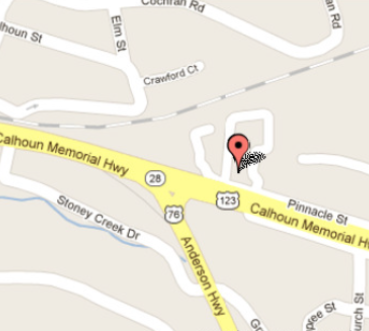
\includegraphics[width=\textwidth]{hotel_map}
\section{Parking}
Visitors \underline{\bfseries must} display a valid guest parking permit to
park on campus except when in areas designated as public parking for a
special event.


We have parking permits that allow you to park in green and orange
marked parking. There is such parking between Sikes (the building on
Calhoun with columns) and Martin Hall, enter along Calhoun Drive and
turn right after Sikes (NOT Cherry Road). You may get permits on Friday
from Martin Schmoll personally (office number Martin O-17), or pick it
up at the conference from room Martin M-105 (Saturday \& Sunday).


Parking permits for visitors can also be obtained from three locations:
\begin{enumerate}
\item The Visitors Center, 109 Daniel Drive
\item Parking Services, G01 Edgar Brown Union
\item Clemson University Police, Memorial
Stadium
\end{enumerate}
\section{Conference Banquet}
The Banquet will be held 6:00 pm -- 7:30 pm in Calhoun Corners
Restaurant located only 1/2 mile from the conference venues at
103 Clemson Street
Clemson, SC 29631
(Phone: (864) 654-7490).

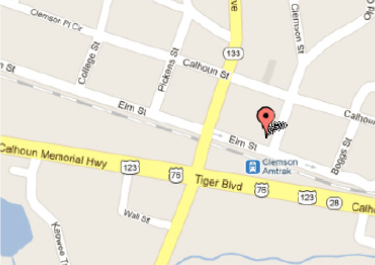
\includegraphics[width=\textwidth]{restaurant_map}

The price, \underline{\bfseries not covered by organizers}, is \$23 and should
be paid in cash upon arrival. The price does not include drinks.



\section{Registration and Financial support} The
conference is partially funded through NSF grant DMS-1201546.  Limited
travel and lodging financial support will be available to the most
attendees. However priority will be given to graduate students,
post-docs and new Ph.D.s. Due to NSF regulations, we kindly ask all
participants to register. If you have not already register please do so
by visiting us at our web site:

\url{http://www.devio.us/~ppunosevac/cdynsys/}


Participants who are requesting financial support will also have to do
vendor registration required by Clemson university as well as to submit
expense report form with receipts.

\section{Organizers}

Martin Schmoll \url{<schmoll@clemson.edu>}

Predrag Puno\v{s}evac \url{<ppunosev@aug.edu>}


\end{document}